\section{Methods}\label{methods}


\subsection{Cloud models}\label{methods:clouds}

\rc{[general comment: In this sub-section I basically copied the descriptions we have used in the previous paper. I am not sure whether the summary given here in to short as I also wanted to provide a summary of the work we have done with the data already. I would appreciate what you think about the structure of this subsection.]}

The analysis in this paper is based on a sample of three molecular clouds (MCs) found within the 3D magnetohydrodynamics~(MHD), adaptive mesh refinement~(AMR) FLASH code \citep{Fryxell2000} simulations by \citet{IbanezMejia2016}.
\citet[hereafter \citetalias{IbanezMejia2016} and \citetalias{IbanezMejia2017}, respectively]{IbanezMejia2016,IbanezMejia2017} and \citet[hereafter \citetalias{Chira2018}]{Chira2018} describe the simulations and the clouds in more details. 
For the context of this paper, we here summarise the most relevant properties. 

The entire 3D MHD AMR simulations model a multi-phase, turbulent interstellar medium (ISM) of a disk galaxy where dense structures form self-consistently in turbulent, convergent flows \citepalias{IbanezMejia2016}. 
The simulations include gravity (stellar potential and dark matter halo, as well as self-gravity after 250~Myr simulated time), supernova-driven turbulence, photoelectric heating and radiative cooling, and magnetic fields. 
The three MCs of our sample are (40~pc)$^{3}$ subregions of the entire $1~\times~1~\times~40$~kpc$^3$ volume.
The authors of \citetalias{IbanezMejia2017} have re-simulated the clouds with an effective spatial resolution of $\Delta x_{\rm min}=0.1$~pc when mapped onto a $400\times 400~\times 400$ grid cells containing cube, respectively.
Substructures of the MCs are fully resolved if their local Jeans length $\lambda_J > 4~\Delta x_{\rm min}$, corresponding to a maximum resolved density of $8~\times 10^3$~cm$^{-3}$ at 10~K \citepalias[e.g.][Eq.~15]{IbanezMejia2017}.
This means that we can trace fragmentation down to 0.4~pc, but cannot fully resolve objects that form at smaller scales.
The MCs have total masses on the order of $3~\times 10^3$, $4~\times 10^3$, and $8~\times 10^3$~M$_{\odot}$ and are denoted as \texttt{M3}, \texttt{M4}, and \texttt{M8}, respectively, hereafter.

This set-up opens opportunities for many different kind of studies. 
The authors of \citetalias{IbanezMejia2017} have described the time evolution of the properties of all three clouds in detail.
In particular focus, the authors have investigated typical observables, such as mass, velocity dispersion, infall velocity and Mach number, in context of MC formation within spiral galaxies.
\citetalias{Chira2018} have studied the properties and time evolution, as well as the fragmentation behaviour of filaments that self-consistently condense within the model clouds. 
The authors have compared their measurements with typical stability criteria in order to evaluate whether they can also be used for predicting fragmentation.

In this paper, we focus on the driving sources of turbulence within the simulated MCs and the signatures they print on observables, such as the velocity structure function.


\subsection{Velocity Structure Functions}\label{methods:vsf}

We probe the power distribution of turbulence throughout the entire simulated MCs by using the so-called velocity structure function (VSF).
The VSF is a two-point correlation function that measures the mean velocity difference, $\Delta \vec{v} = \vec{v}(\vec{x}+\vec{\ell}) - \vec{v}(\vec{x})$, between two grid cells $\vec{x}$ and $\vec{x}+\vec{\ell}$ (with $\vec{\ell}$ being the direction vector pointing from the first to the second cell), to the $p^\mathrm{th}$ power as function of lag distance, $\ell = |\vec{\ell}|$, between the correlated points.
Thereby, the VSF estimates the occurrence of symmetric motions (e.g., rotation, collapse, outflows), as well as rare events of random turbulent flows (e.g., SNe) in velocity patterns.
Those patterns become more prominent the higher order $p$ is \citep{Heyer2004}.

For data on an Eulerian grid, such as ours, the density-weighted definition of the VSF, $\mathit{S}_p$, is given by
\begin{equation}
	\mathit{S}_p (\ell) = \frac{\langle \, \rho(\vec{x}) \rho(\vec{x}+\vec{\ell}) \, |\Delta \vec{v}|^p  \, \rangle}{\langle  \, \rho(\vec{x}) \rho(\vec{x}+\vec{\ell}) \, \rangle} ,
    \label{equ:method:def_vsf}
\end{equation}
\citep[and references within]{Padoan2016a}.
With this definition one can see that each order of the VSF has a physical meaning. 
For example, $\mathit{S}_1$ is to the mean relative velocities between cells, reflecting the modes created by different gas flows.
$\mathit{S}_2$ is proportional to the kinetic energy, making it a good probe of how the turbulent energy is transported to different scales.

If the turbulence is fully developed the VSF is supposed to be well-described by a power-law relation \citep{Kolmogorov1941,She1994,Boldyrev2002}:
\begin{equation}
	\mathit{S}_p (\ell) \propto \ell^{\zeta(p)} .
    \label{equ:method:propto_zeta}
\end{equation}
Note that the scaling exponent of that power-law relation, $\zeta$, depends on many parameters, such as the order of the VSF, as well as the properties and composition of the studied turbulent flow, like its geometry, compressibility or Mach number.
Many studies on VSFs distinguish between longitudinal and transverse velocity components, or compressible and solenoidal gas flow components because those are expected to behave differently, especially towards larger lag distances \citep{Gotoh2002,Schmidt2008,Benzi2010}.
However, the differences are mostly negligible on the scales we focus on. 
This and the fact that those components are observationally very hard to differentiate are the reasons why we analyse all components in a common sample.

There are some theoretical studies that predict values of $\zeta$ depending on the nature of turbulence and the order $p$.
For example, \citet{Kolmogorov1941} predicts that the third-order exponent, $\zeta(3)$, is equal unity for an incompressible, transonic flow.
This results in the commonly known prediction that the kinetic energy decays with $E_k(k) \propto k^{-\frac{5}{3}}$, with $k = \frac{2 \pi}{\ell}$ being the wavenumber of the turbulence mode.

For a supersonic flow, however, it is always supposed to be greater or equal to unity.
Based on \citeauthor{Kolmogorov1941}'s work, \citet{She1994} and \citet{Boldyrev2002} have extended and generalised the analysis and predict the following.
For an incompressible filamentary flow \citet{She1994} predict that the VSFs scale with,
\begin{equation}
	\zeta_\mathrm{She}(p) = \frac{p}{9} + 2 \left[ 1 - \left( \frac{2}{3} \right)^{\frac{p}{3}} \right] = Z_\mathrm{She}(p) ,
    \label{equ:method:she}
\end{equation}
while supersonic flows with sheet-like geometry are supposed to scale with \citep{Boldyrev2002},
\begin{equation}
	 \zeta_\mathrm{Boldyrev}(p) = \frac{p}{9} + 1 - \left( \frac{1}{3} \right)^{\frac{p}{3}} = Z_\mathrm{Boldyrev}(p) .
    \label{equ:method:boldyrev}
\end{equation}
\citet{Benzi1993} have introduced the principle of "extended self-similarity".
It proposes that there is a constant relationship between the scaling exponents of different orders on all lag scales. Normally, the self-similarity parameter, $Z$, normally refers to the 3$^mathrm{rd}$ order VSF and is given by:
\begin{equation}
	Z(p) = \frac{\zeta(p)}{\zeta(3)} .
	\label{equ:method:z_def}
\end{equation} 
Since the mentioned predictions of $\zeta(p)$ are normalised in a way that $\zeta(3)$~=~1 Eq.~(\ref{equ:method:she}) and~(\ref{equ:method:boldyrev}) also provide the predictions for $Z(p)$, respectively.

For the discussion below, we measure $\zeta$ by fitting a power-law, given by
\begin{equation}
	\log_{10}\left[ S_p(\ell) \right] = \log_{10}\left(A\right) + \zeta \log_{10}(\ell) ,
    \label{equ:method:fitting}
\end{equation}
with $A$ being the proportionality factor of the power-law to the simulated measurements.
For the calculations, we only take those cells with a minimal number density of 100~cm$^{-3}$ into account as this threshold defines the volume of the clouds.
For reducing the computational effort we divide the range of 3D lag distances, $\ell$, into 40 equidistantly separated bins ranging from~0.1 to 30~pc.
This means that the measurements at the given lag interval $\ell_i$ we will show below base on the data with lag distances $\ell_{i-1} < \ell \leq \ell_i$.

Fig.~\ref{pic:results:vsf_example} shows three examples of VSFs, namely (a) \texttt{M4} $t$~=~1.2~Myr, after self-gravity has been activated in the simulations, (b) \texttt{M3} at $t$~=~3.5~Myr, and (c) \texttt{M3} at $t$~=~4.0~Myr.
All plots illustrate the VSFs of the orders $p$~=~1--3 that are computed based on the simulation data.
The solid lines show the fitted power-law relations as given in Eq.~(\ref{equ:method:fitting}).

\begin{figure*}[!htb]
	\centering
	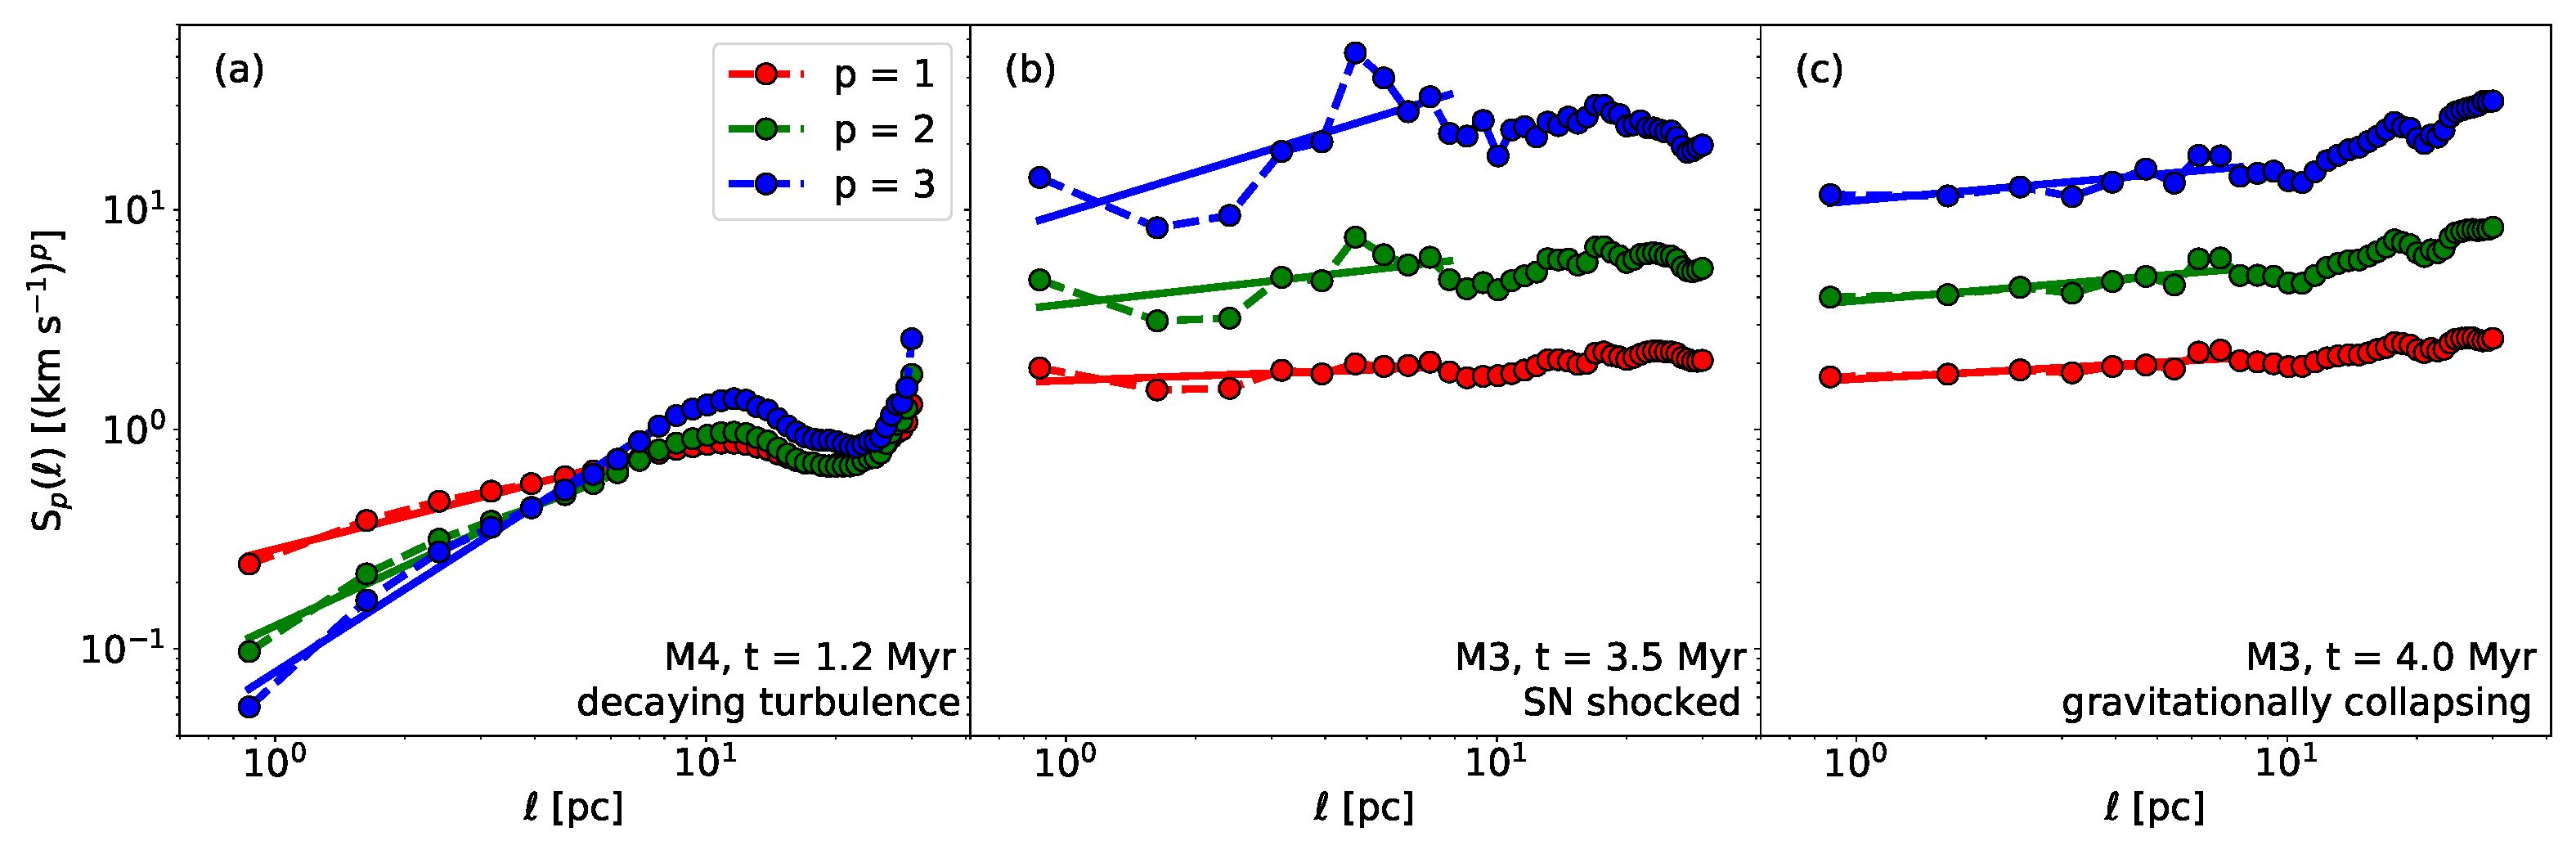
\includegraphics[width=\textwidth]{vsf_example.pdf}
    \caption{Examples of velocity structure functions as function of the lag scale, $\ell$, and order, $p$. 
    	The dots (connected by dashed lines) illustrate the measured values based on the simulation data. 
        The solid lines represent the power-law relations fitted to the respective structure function.
	}
    \label{pic:results:vsf_example}
\end{figure*}

The examples demonstrate that, in general, the measured VSFs cannot be described by a single power-law relation over the entire range of $\ell$.
Instead they are composed of roughly three different regimes: 
one at small scales at $\ell \lesssim$~3~pc, a second one within 3~pc~$\lesssim \ell \lesssim$~10--15~pc, and the last one at large scales with $\ell >$~15~pc.
Therefore, only the small and intermediate ranges may be represented by a common power-law relation.
On larger scales, one observes a local minimum before the VSFs either increase or stagnate.
The location of the minimum, thereby, coincides with the equivalent radius of the cloud, meaning the radius a cloud of given mass would have if it would be a sphere.
Thus, in this context the VSF is an accurate tool to measure the size of a molecular cloud.
On smaller scales, which correspond to individual clumps and cores, one sees significant differences.

The examples in Fig.~\ref{pic:results:vsf_example} illustrate how the clouds and their VSFs react to different scenarios that affect the turbulent structure of the entire clouds. 
In Fig.~\ref{pic:results:vsf_example}a one sees the standard case where turbulence is fully developed, driven on large scales and decays to small scales.
This is the dominant case within the first $\sim$1.5~Myr of the simulations.
During this interval of time the clouds experience the effect of self-gravity for the first time in their evolution and need to adjust to this new condition.
Until this is the case, their VSFs are dominated by the freely cascading turbulence that previously dominated the kinetic structure of the clouds.
Furthermore, this implies that we can only reliably examine turbulence within the simulations after 1.5~Myr and carefully need to take this into account in the further discussion \citep[see][]{IbanezMejia2017,Seifried2017b}.

The other examples represent the clouds at later stages of their evolution when the VSFs are dominated by sources that drive the turbulence within the clouds in a more extreme way.
Fig.~\ref{pic:results:vsf_example}b shows the VSF of \texttt{M3} at a time when the cloud has just been hit by a supernova (SN) shock front. 
One clearly sees how the amplitude of the VSFs is increased by one to two orders of magnitudes compared to the previous example.
Especially the power of small scale turbulence ($\ell \lesssim$ few parsecs) is highly amplified as result of the shock, while it reduces the equivalent radius of the cloud.
Despite the increase of turbulent power at small scales, there is a great amount of energy injected at large scales, as well.
All this results in a steeper scaling of the VSF.
However, the effect of SN shocks last for only a short period of time (see below).

The last example, Fig.~\ref{pic:results:vsf_example}c, demonstrates the imprint of gravitational contraction.
Here, the VSF is almost flat, or even slightly increasing towards smaller separation scales. 
This kind of profile is typical for gas that is self-gravitationally contracting \citep{Boneberg2015,Burkhart2015} since gas moves into the inner regions of the cloud, reducing the average lag distances, but not necessarily the relative velocities.
The latter may even be accelerated by the infall.
As a consequence, large amounts of kinetic energy are transferred to smaller scales which flattens the corresponding VSF.


\endinput
